\section{Periféricos Principales}
\label{sec:perif}

\begin{itemize}
\item Microcontrolador ATMega32: Es el periférico central de este trabajo. Toda la información entra o sale por el mismo y es el encargado de interconectar al resto de los periféricos entre sí. Algunos de los motivos por los cuales se eligió este microcontrolador entre la diferente variedad que ofrece Atmel son:

\begin{itemize}
\item Posee la cantidad de pines suficiente para poder conectar el resto de los periféricos.
\item La cantidad de memoria RAM y ROM que posee resulta más que suficiente para poder almacenar una tabla de las funciones pre cargadas y también para guardar en memoria volátil las muestras de una función periódica que se envía desde Matlab.
\item Cuenta con el protocolo USART.
\item Tiene un conversor analógico-digital integrado, el cual se utiliza para poder medir la intensidad haciendo uso del módulo de detección. Esto se debe a que dicho módulo transforma la intensidad del haz que incide sobre el mismo en un valor de tensión (señal analógica).
\item Al ser frecuentemente utilizado en sistemas embebidos, es posible encontrar en internet información y documentación sobre cómo utilizar cada una de las funciones que posee, en contraposición a otros tipos de microcontroladores.
\end{itemize}

\begin{figure}[H]
  \centering
  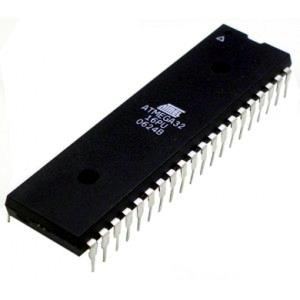
\includegraphics[width=0.5\textwidth]{images/atmega32.jpg}
  \caption{Microcontrolador ATmega32}
  \label{fig:atmega32}
\end{figure}

\item Placa conversora USB a Serie, necesaria para poder conectar a una computadora va puerto USB y que la computadora sea capaz de reconocer al dispositivo como un puerto serie virtual. De esta manera es posible utilizar las funciones de Matlab que permiten enviar datos a través de un puerto serie. Además estas placas incluyen conexiones para alimentar al microcontrolador con lo cual se lo podría energizar solamente con la conexión a una computadora sin necesidad de utilizar un cable adicional. En el mercado argentino se encuentran este tipo de placas basadas en dos integrados distintos: Cp2102 y CH340. De estos dos se utilizó una placa basada en Cp2102 ya que era la de menor costo.

\begin{figure}[H]
  \centering
  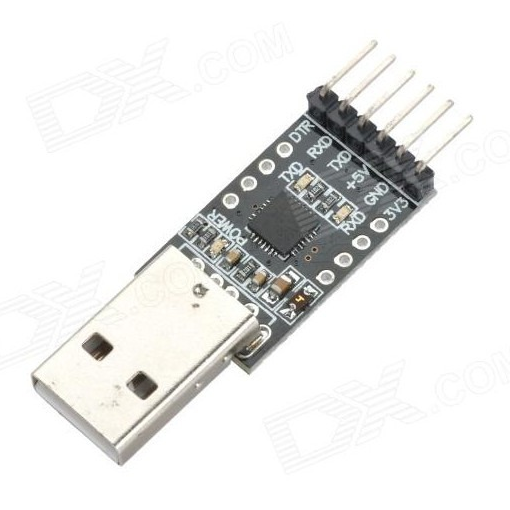
\includegraphics[width=0.5\textwidth]{images/conversor_usbttl.png}
  \caption{Ejemplo de placa conversora usb a serie}
  \label{fig:usbattl}
\end{figure}


\item Red R2R: Se trata de una implementación sencilla de un conversor digital-analógico (DAC). Tal cual indica su nombre, R2R (también conocido como escalera de resistencias), se trata de un circuito electrónico formado por resistencias alternando dos valores posibles, donde un valor debe ser el doble del otro. Tiene como ventajas su fácil implementación, su conversión eficiente y la independencia que presenta en comparación con DACs integrados, donde estos últimos necesitan varias fuentes de alimentación, donde en algunos casos dichos valores de alimentación son atípicos.

\item Display LCD: Es necesario para para poder visualizar las opciones a elegir, para  definir el tipo de desplazamiento desde el microcontrolador.
\begin{figure}[H]
  \centering
  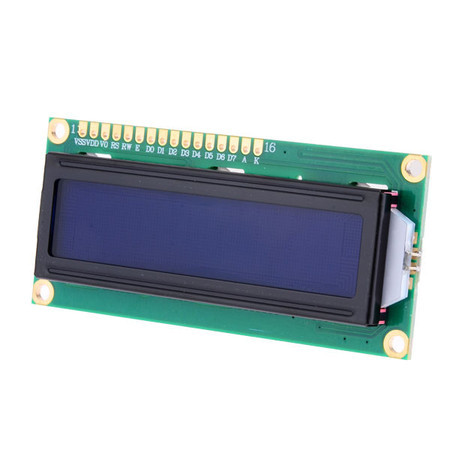
\includegraphics[width=0.6\textwidth]{images/displayLCD.jpg}
  \caption{Ejemplo Display LCD 16x2}
  \label{fig:display}
\end{figure}
\item Pulsadores: Son necesarios para seleccionar el tipo de desplazamiento a efectuar, donde las opciones serán visualizadas en el display.
\item Parlante o Altavoz: Necesario para poder generar el desplazamiento en el espejo. Será necesario evaluar distintos tipos de parlantes para entender cuál resulta útil para cumplir nuestros objetivos.
%\item Diseñar un soporte para el dispositivo en su totalidad de manera tal que pueda ser utilizado en una mesa antivibratoria en la cual se encuentra instalado el interferómetro. En este soporte estará colocado el parlante con un espejo pegado al mismo.
\end{itemize}